\documentclass[letterpaper,titlepage]{article}

%%%%%%%%%%%%%%%%%%%%%%%%%%%%%%%%%%%%%%%%
% Config
%%%%%%%%%%%%%%%%%%%%%%%%%%%%%%%%%%%%%%%%

% Page layout, header, footer
\usepackage{fullpage}
%\usepackage{indentfirst}
%\setlength{\parindent}{0pt}
	
% For graphics
\usepackage{graphicx}
\graphicspath{{./gfx/}}
\usepackage{wrapfig}

% For URLs
\usepackage[colorlinks,
            linkcolor=black,
            filecolor=black,
	            urlcolor=black]
            {hyperref}

\usepackage{fancyhdr}
\setlength{\headheight}{15pt}
\setlength{\headsep}{25pt}
\pagestyle{fancy}
	
\fancyhf{} % clear all header and footer fields
\fancyhead[L]{Software Design Description}
\fancyfoot[L]{\today}
\fancyfoot[C]{Section \thesection}
\fancyfoot[R]{\thepage}
\renewcommand{\headrulewidth}{0.4pt}
\renewcommand{\footrulewidth}{0.4pt}

% Signature Stuff
\newcommand{\sigline}[1]{
  \rule{\textwidth}{.5pt}\\
  \begin{tabular*}{\textwidth}{@{\extracolsep{\fill}} l r }
  #1 & Date\\[2.5cm]
  \end{tabular*}
}
	
% Shortcut commands
\newcommand{\bullets}[1]{\begin{itemize} #1 \end{itemize}}
\newcommand{\deflist}[1]{\begin{description} #1 \end{description}}
	
\begin{document}
\pagenumbering{roman}

%%%%%%%%%%%%%%%%%%%%%%%%%%%%%%%%%%%%%%%%
% Title Page
%%%%%%%%%%%%%%%%%%%%%%%%%%%%%%%%%%%%%%%%
\title{\textbf{Software Design Description}}
\author{\textbf{Windmill Software }\\
        Steven Cornella \\ Armon Entezari \\ Dustin Ingram \\ Aaron Rosenfeld \\ Michael Vadovszki
	}
\date{\today\\Revision 0}
\maketitle
\pagebreak

%%%%%%%%%%%%%%%%%%%%%%%%%%%%%%%%%%%%%%%%
% Contents
%%%%%%%%%%%%%%%%%%%%%%%%%%%%%%%%%%%%%%%%
\thispagestyle{plain}
\setcounter{tocdepth}{3}
\tableofcontents
\pagebreak

%%%%%%%%%%%%%%%%%%%%%%%%%%%%%%%%%%%%%%%%
% Body
%%%%%%%%%%%%%%%%%%%%%%%%%%%%%%%%%%%%%%%%
%\setcounter{page}{1}
\pagenumbering{arabic}

\newcommand{\defn}[2]{\paragraph{#1}{#2}}
\section{Introduction}
\subsection{Purpose}
The purpose of this document is to explain all necessary requirements for Windmill's chess software in the
IEEE standard. This include functional, non-functional, constraints, use case specifications, and graphical prototypes
of our chess software.

\subsection{Scope}
This document is the initial version (1.0) of the requirements specifications for Windmill's chess software. Software
developers and testers are the intended readers of this document.

\subsection{Definition, Acronyms, and Abbreviations}
\defn{Bishop}{One of six chess pieces in a chess game. It is permitted to only move in a diagonal direction on a
chessboard.}
\defn{Checkmate}{A chess game state wherein one player's king will be inevitably captured.}
\defn{Chess}{A board game played between two players on a chess board with sixty four squares. Each square may hold only
one chess piece.}
\defn{GUI}{Acronym for Graphical User Interface. It provides a graphical front end for computer programs.}
\defn{Internet}{A large worldwide system of connected networks.}
\defn{IP Address}{Unique 32-bit number that identifies any computer connected to the Internet.}
\defn{Port}{A 16-bit number that indicates a communication channel on a specific machine.}
\defn{Java}{An object oriented computer programming language.}
\defn{King}{One of six chess pieces in a chess game. Each player receives one king at the start of the chess game. It can
move in any direction on a chessboard. The objective in a chess game is to protect it from capture by the opponent.}
\defn{Knight}{One of six chess pieces in a chess game. Each player receives two knights at the start of the chess game. It
moves in two possible unique ways, two horizontally and one vertically or vice versa.}
\defn{Queen}{One of six chess pieces in a chess game. Each player receives one queen at the start of the chess game. In a
chess game, it can move in any direction.}
\defn{Rook}{One of six chess pieces in a chess game. Each player receives two rooks at the start of the chess game. It can
move either horizontally or vertically any number of squares.}
\defn{Swing}{An API library for providing a GUI to Java programs.}
\defn{Thread}{Code that runs within the address space of a single process.}

\subsection{Overview}
Following this introduction, an overall description, use case diagrams, non-functional and functional requirements, and graphical user
interface prototypes are presented.



\section{Static Design Structure Modeling}
For a larger version, please see the included file ``class-diagram.pdf''.
\begin{center}
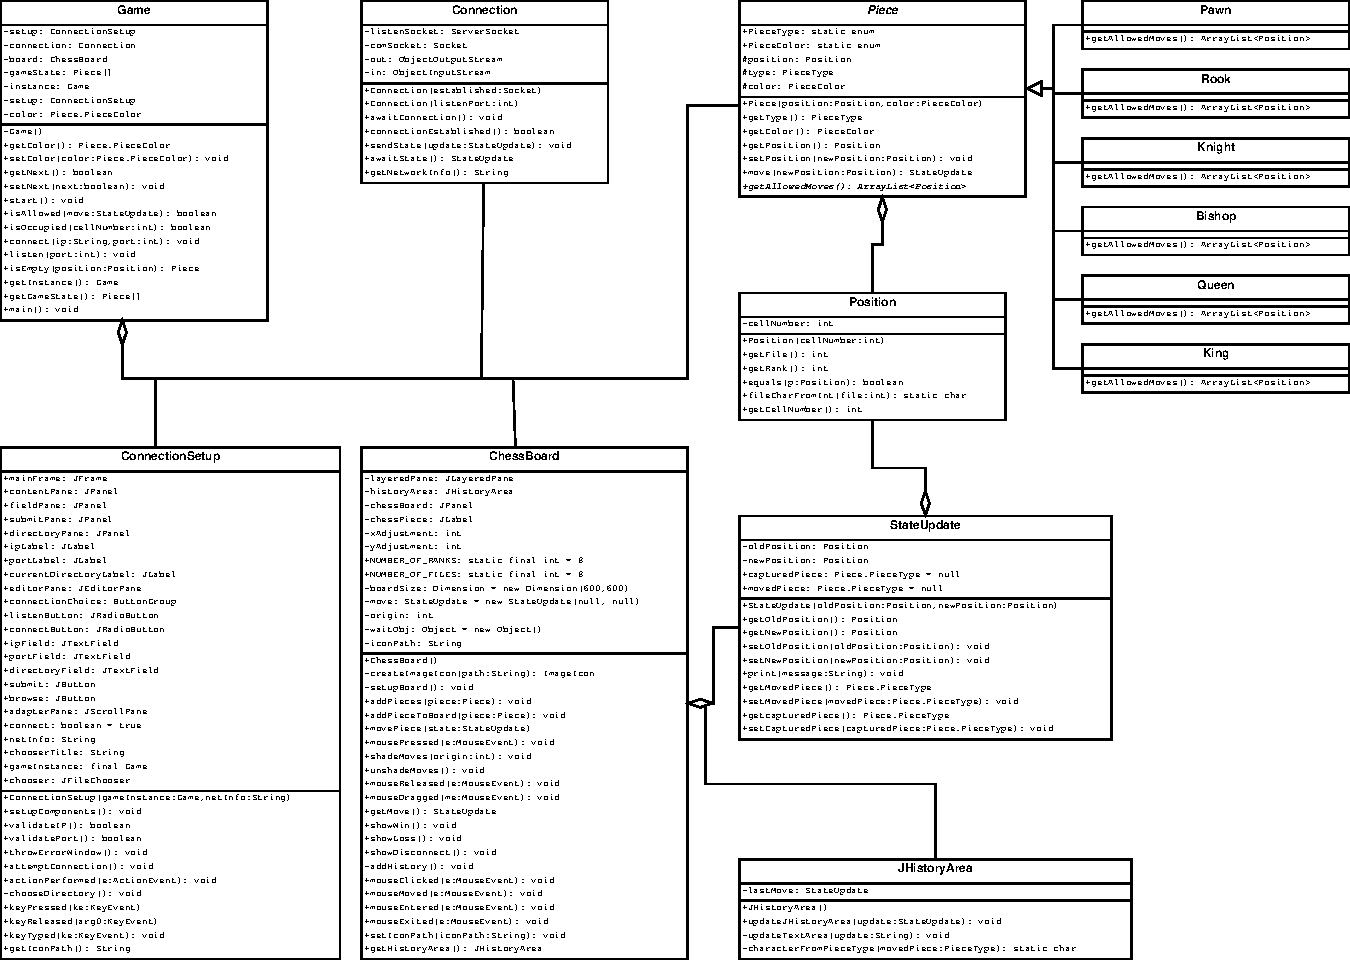
\includegraphics[scale=.7]{class-diagram.pdf}
\end{center}

\section{Dynamic Behavior Modeling}

\subsection{Start New Game}
\begin{center}
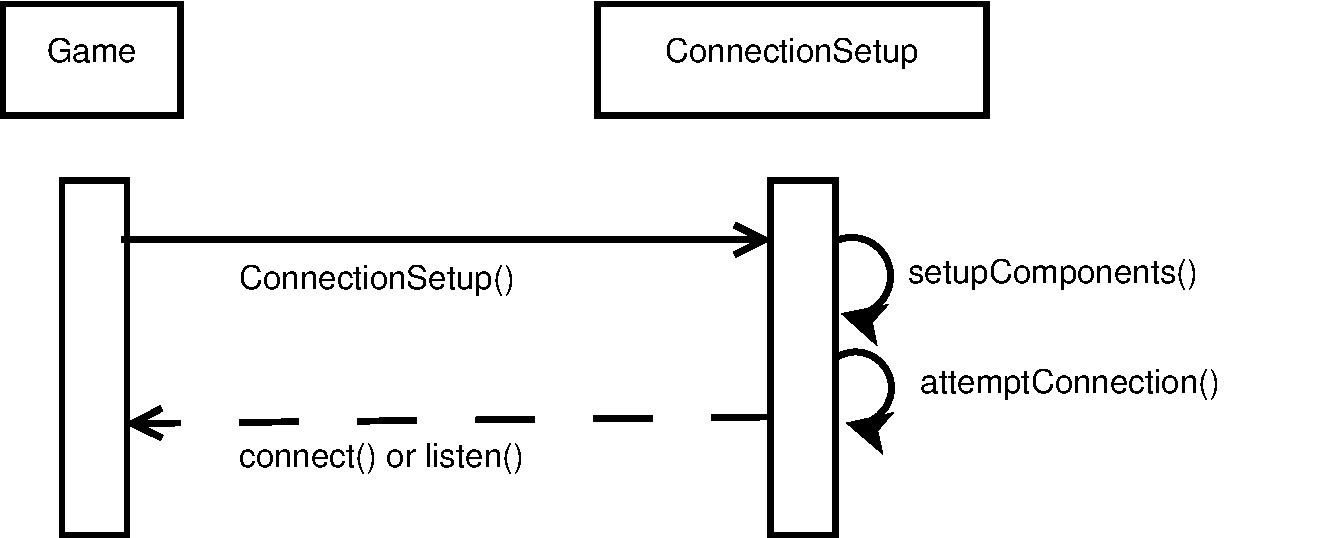
\includegraphics[scale=.50]{StateDiagrams/StartNewGame.pdf}
\end{center}

\subsection{Wait for Opponent Connection}
\begin{center}
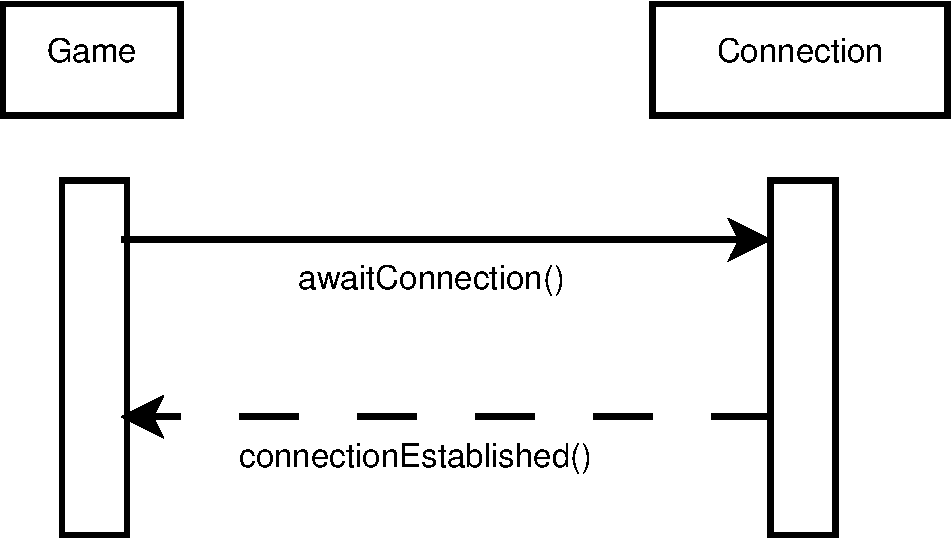
\includegraphics[scale=.50]{StateDiagrams/WaitForOpponentConnection.pdf}
\end{center}

\subsection{Connect to Opponent} \label{sec:connect}
\begin{center}
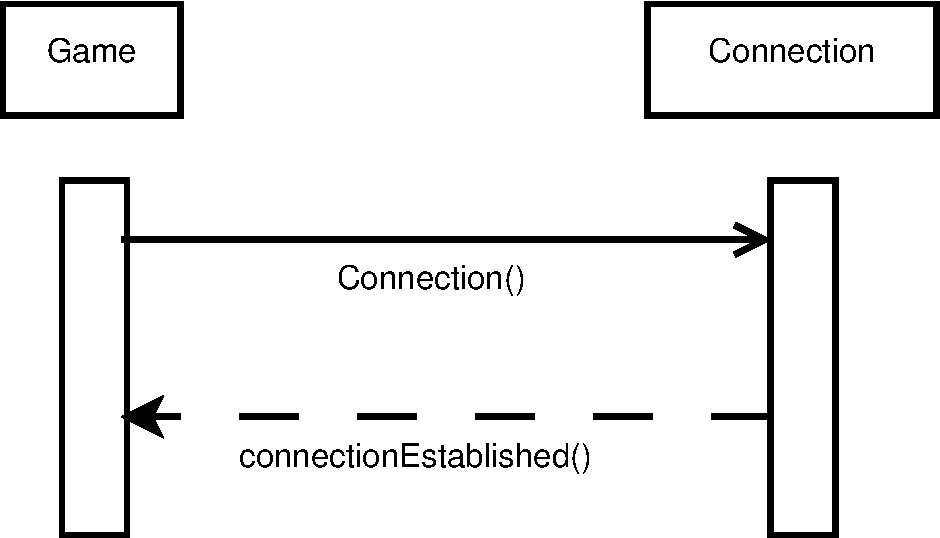
\includegraphics[scale=.50]{StateDiagrams/ConnectToOpponent.pdf}
\end{center}

\subsection{Move Piece} \label{sec:move-piece}
\begin{center}
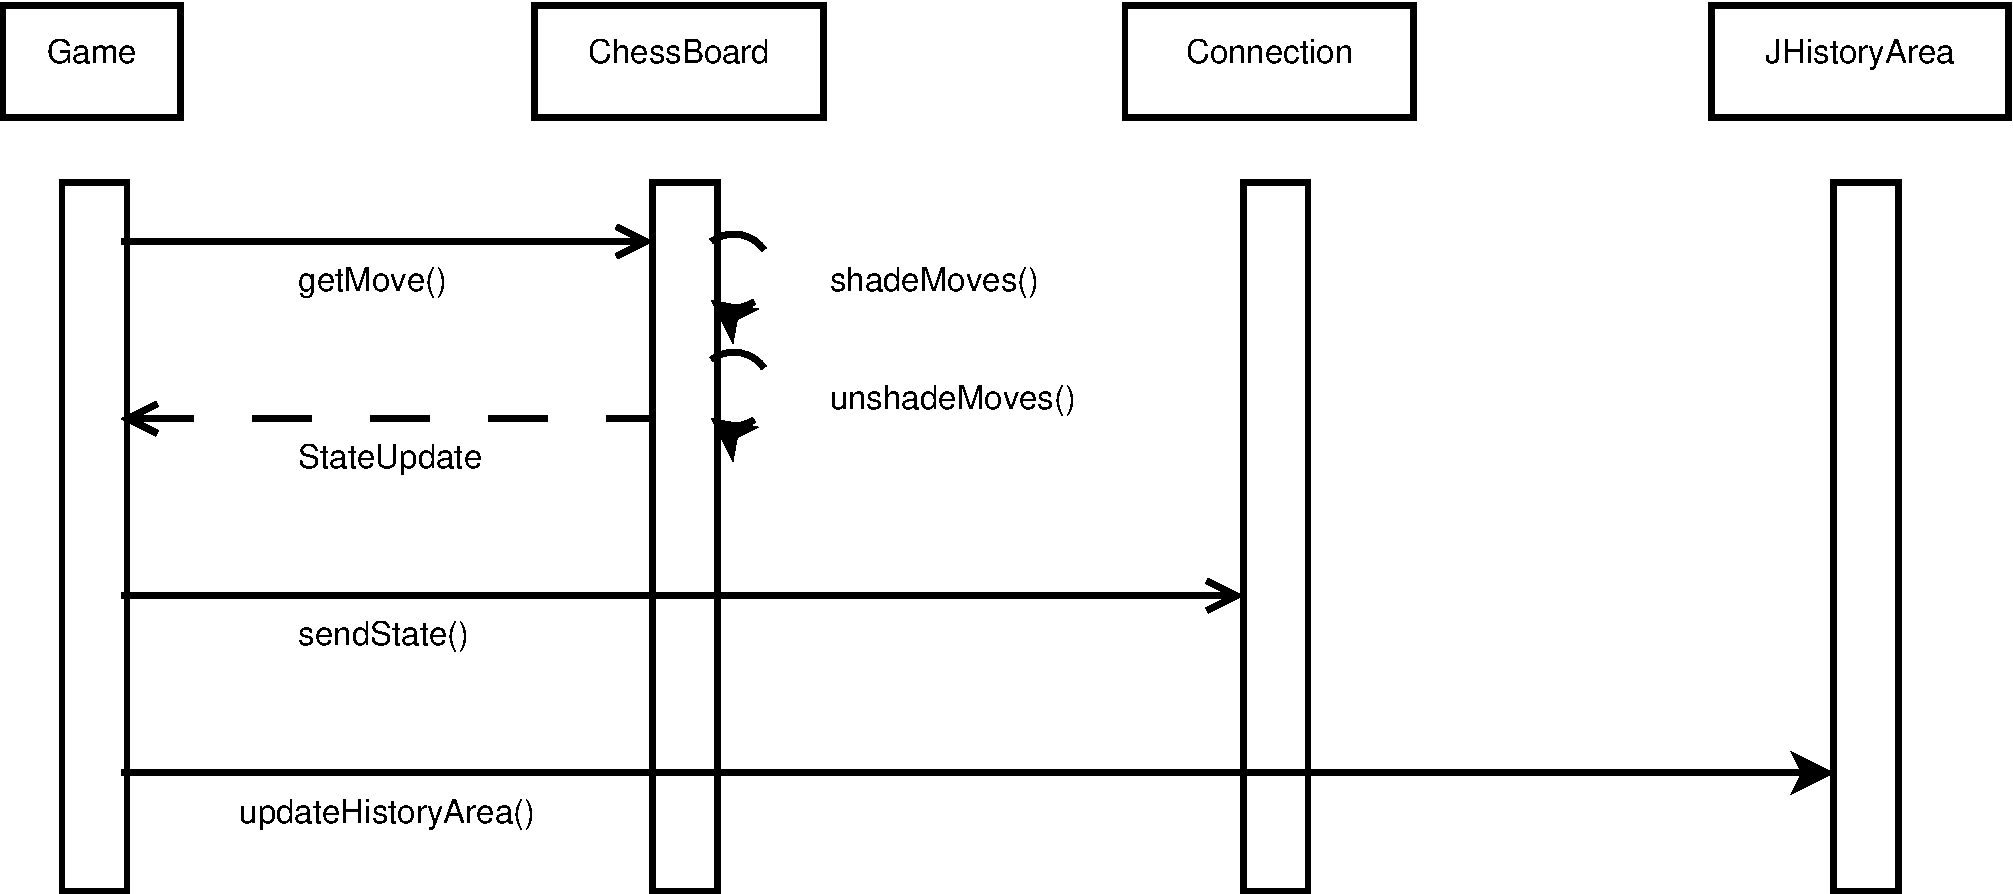
\includegraphics[scale=.50]{StateDiagrams/MovePiece.pdf}
\end{center}

\subsection{Wait for Opponent Move}
\begin{center}
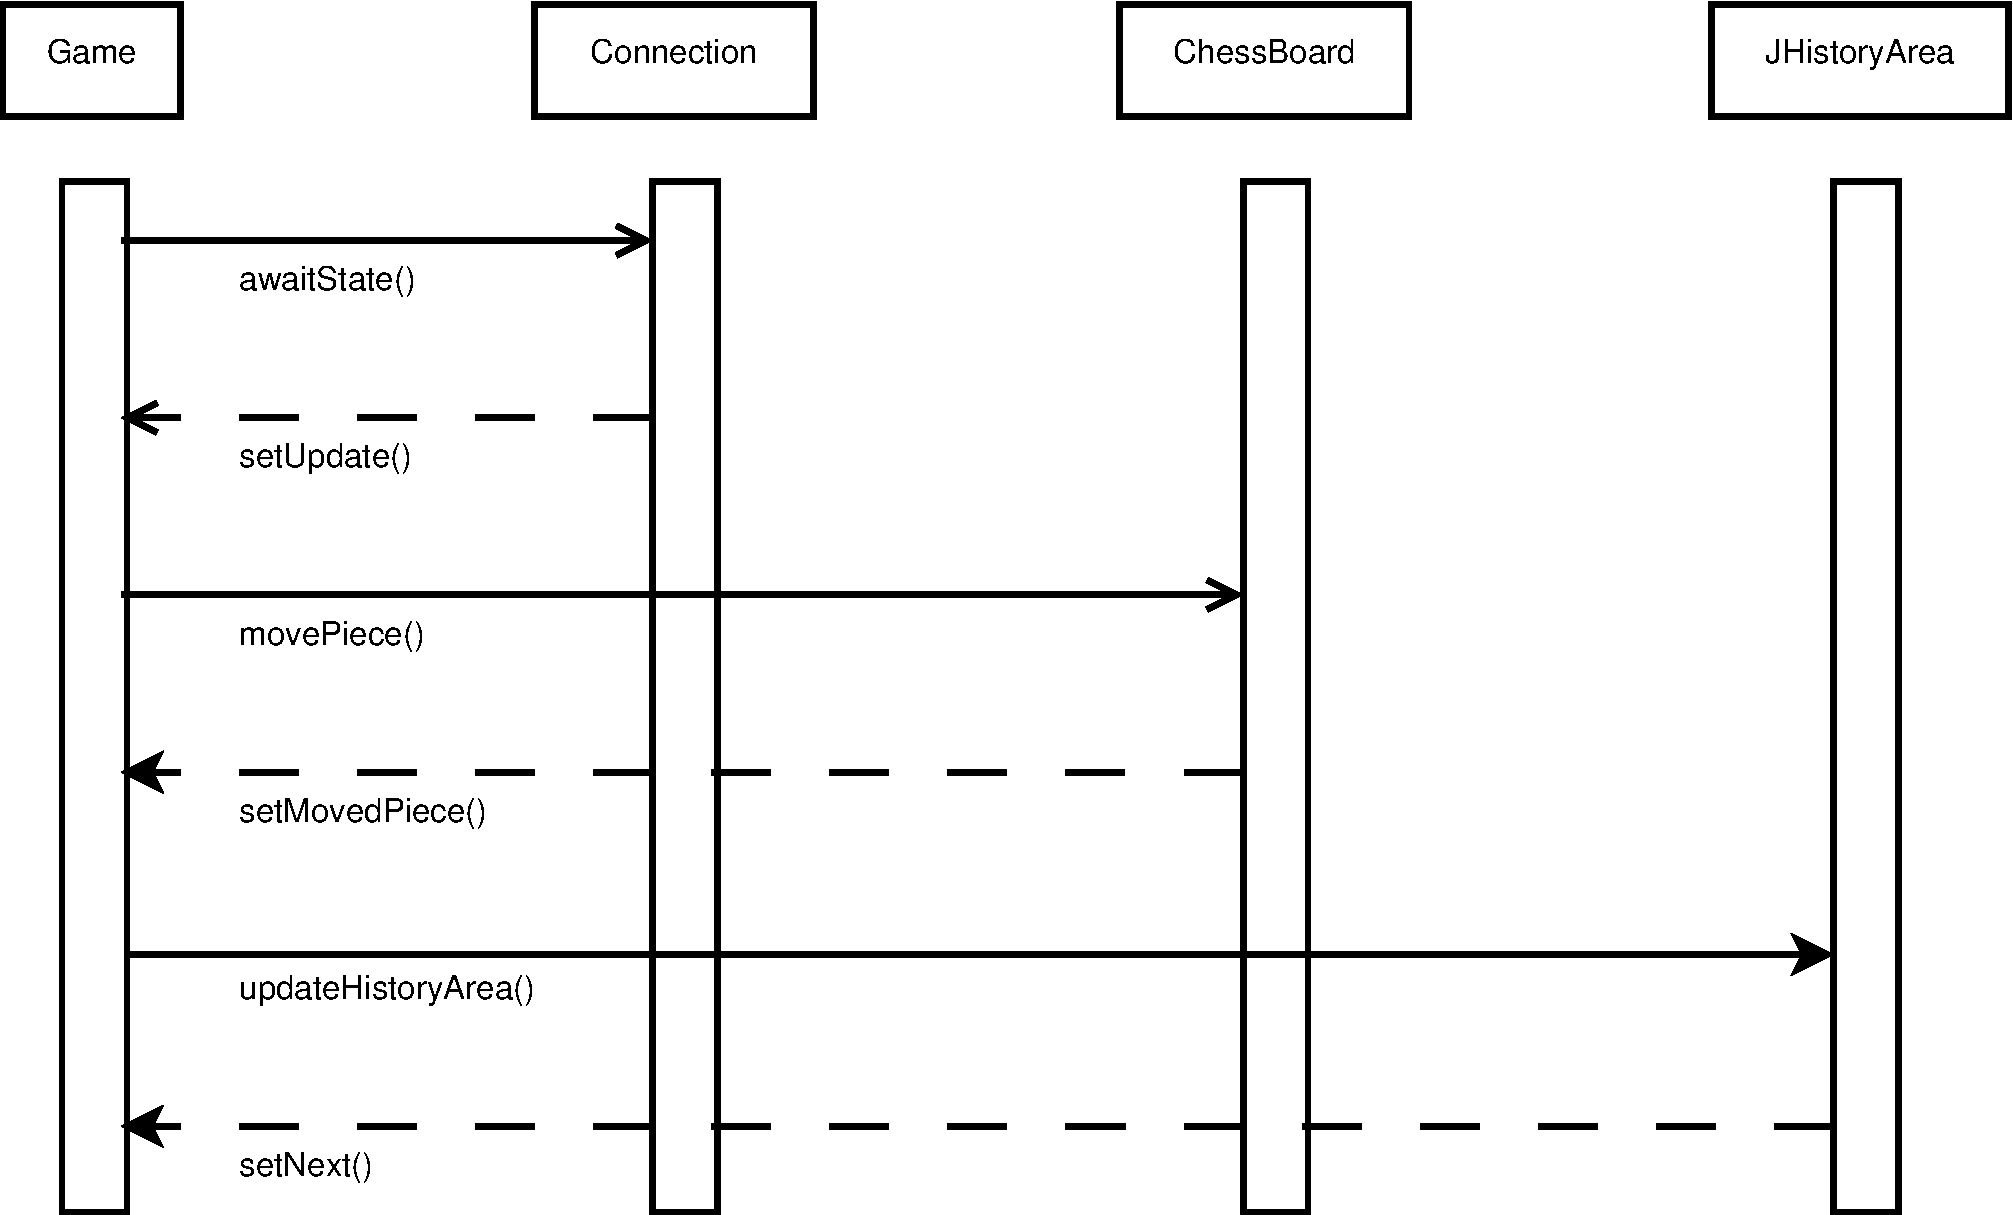
\includegraphics[scale=.50]{StateDiagrams/WaitForOpponentMove.pdf}
\end{center}

\subsection{Game End} \label{sec:game-end}
\begin{center}
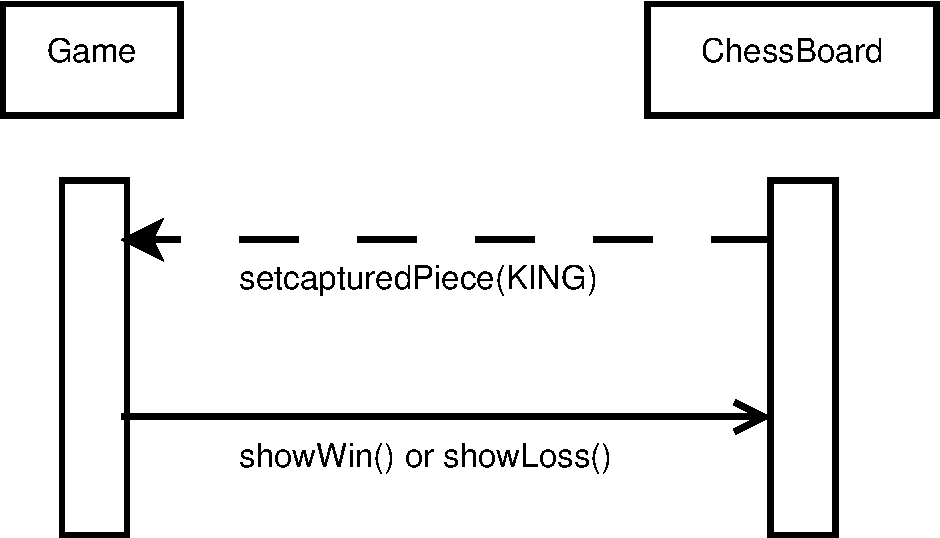
\includegraphics[scale=.50]{StateDiagrams/GameEnd.pdf}
\end{center}

\subsection{Change Game Icons} \label{sec:icons}
\begin{center}
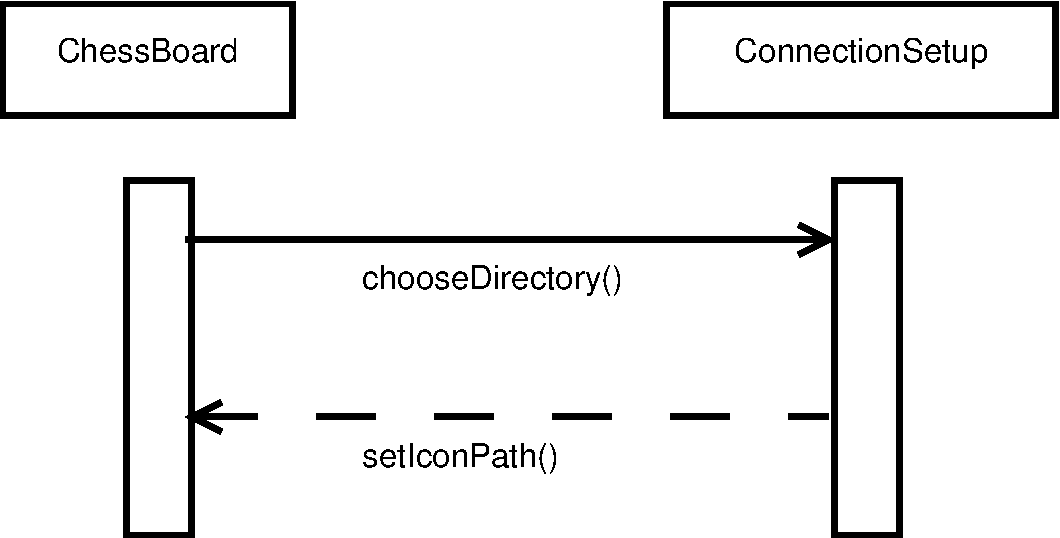
\includegraphics[scale=.50]{StateDiagrams/ChangeGameIcons.pdf}
\end{center}

\section{Requirement Traceability Table}

\begin{center}
\begin{tabular}{|c|c|}
    \hline
    \textbf{Requirement} & \textbf{Component} \\ \hline
    Handle special chess moves & \ref{sec:move-piece} \\ \hline
    Modify piece icons & \ref{sec:icons} \\ \hline
    Log moves in algebraic notation & \ref{sec:move-piece} \\ \hline
    Notify when game has ended & \ref{sec:game-end} \\ \hline
    Specify a specific IP/port for game-play & \ref{sec:connect} \\ \hline
\end{tabular}
\end{center}

\end{document}

